%TCIDATA{LaTeXparent=0,0,relatorio.tex}
\ifx\compilewholereport\undefined
	\documentclass[11pt,a4paper,oneside]{book}
	
	% Escolher um dos seguintes formatos:
	\usepackage{ft2unb} % segue padrão de fontes do Latex
	
	% Pacotes
	\usepackage{graphicx}
	\usepackage{amsfonts}
	\usepackage{amsmath}
	\usepackage{amssymb}
	\usepackage[thmmarks,amsmath]{ntheorem}
	\usepackage{boxedminipage}
	\usepackage{theorem}
	\usepackage{fancybox}
	\usepackage{fancyhdr}
	\usepackage{url}
	\usepackage{afterpage}
	\usepackage{xcolor}
	\usepackage{rotating}
	\usepackage{makeidx}
	\usepackage{indentfirst}
	\usepackage{subcaption}
	\usepackage{todonotes}
	\usepackage{listings}
	\presetkeys{todonotes}{inline}{}
	
	\begin{document}
	\frontmatter
	\listoftodos
	\tableofcontents
	\mainmatter
	
	%%%%%%%%%%%%%%%%%%%%%%%%%%%%
	%%%%%%%% Apagar coisas acima
	%%%%%%%%%%%%%%%%%%%%%%%%%%%%
	\newcommand\dlq{\lq\lq{}}
	\newcommand\drq{\rq\rq{}}
\fi

\lstdefinestyle{customVHDL}{
	  belowcaptionskip=1\baselineskip,
	  breaklines=true,
	  frame=l,
	  xleftmargin=\parindent,
	  language=VHDL,
	  showstringspaces=false,
	  basicstyle=\footnotesize\ttfamily,
	  keywordstyle=\itshape\color{blue!40!black},
	  commentstyle=\itshape\color{blue!40!black},
	  identifierstyle=\itshape\color{blue!40!black},
	  stringstyle=\itshape\color{blue!40!black},
}
                      
\chapter{Desenvolvimento}\label{CapDesenvolvimento}

\resumodocapitulo{Este capítulo trata da concepção dos experimentos realizados. Nele serão descritos com detalhes cada um dos experimentos, ficando a parte de análise reservada ao capítulo \ref{CapExperimentos}.}

\section{Introdu\c{c}\~{a}o}
%\vspace{0.8cm}
Devido ao caráter experimental e exploratório do objetivo proposto na seção \ref{sec:projeto}, decidiu-se dividir o projeto em vários experimentos menores.
Desta forma, além de garantir algum material mesmo que tudo dê errado, consegue-se simplificar o processo de pesquisa e desenvolvimento através dos pequenos passos e análises frequentes.

Como o objetivo final do projeto é a familiarização com as ferramentas e processos envolvidos na autoreconfiguração, decidiu-se começar estudando os elementos necessários para se realizar a reconfiguração dinâmica.
O passo seguinte mais lógico é o de estudar como funciona as memórias dos sistema e de que jeito elas seriam melhor utilizadas.
O último passo seria entender como funciona a autoreconfiguração em baixo nível, ou seja, como os dados devem ser entregues aos devidos componentes para que ela aconteça.
Para cada um destes experimentos foi proposto um teste que validasse o completo entendimento do mesmo.

\begin{figure}[h]
\centering
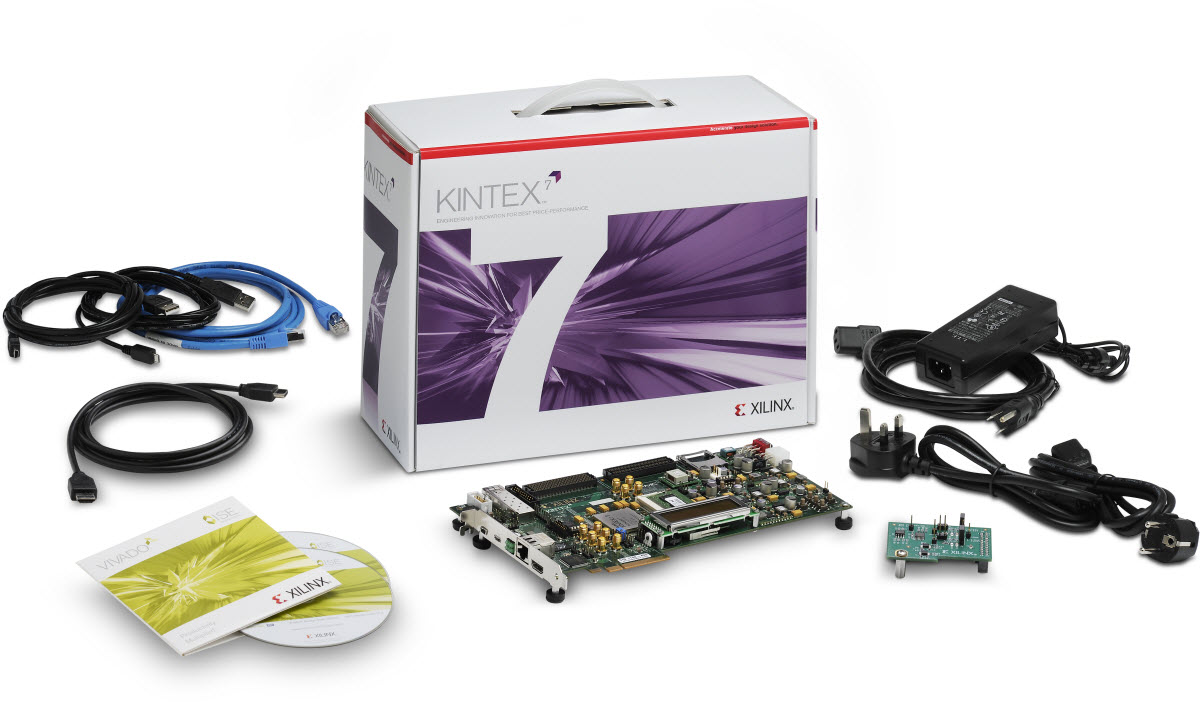
\includegraphics[width=0.7\textwidth]{fig/c3_desenvolvimento/intro/kintex-7_kc705}
\caption{Foto ilustrativa do kit de desenvolvimento Kintex-7 KC705 extraida do site da Xilinx.}
\label{fig:kc705}
\end{figure}

Para o desenvolvimento desse projeto, escolheu-se utilizar o kit de desenvolvimento da Xilinx\textregistered{} chamado Kintex-7 KC705.
O único critério utilizado foi a disponibilidade dos equipamentos no início do projeto e a capacidade do dispositivo de realizar a reconfiguração parcial dinâmica.
Este kit possui FPGA modelo XC7K325T-2FFG900C, leitor de cartão de memória, conector PCIe\textregistered{}, memória DDR3, visor de 7-segmentos e porta ethernet, dentre outros.

Escolheu-se ainda, de forma arbitrária, o uso da linguagem VHDL para a descrição de \textit{hardware} ao invés da Verilog.

\section{Experimento 1 - Reconfiguração Dinâmica}
De forma a dar validade a todo o projeto, foi preciso desenvolver um experimento para se entender o processo de desenvolvimento de sistemas reconfiguráveis dinamicamente e algumas peculiaridades do kit de desenvolvimento.

\subsection{Fluxo de Ferramentas}
A primeira coisa que se destaca no desenvolvimento de dispositivos dinamicamente reconfiguráveis é a diferença no fluxo de ferramentas, também conhecido como \textit{software tools flow}, em relação ao fluxo tradicional \cite{ug743}.
Esta diferença é motivada pela necessidade de construção de diversos \textit{bitfiles} parciais.
Como pode-se ver da figura \ref{fig:ex1:softwareflow}, o fluxo tradicional requer apenas o uso do programa ISE, e opcionalmente do XPS e do SDK, para a construção de um projeto de \textit{hardware} e o iMPACT para a programação da FPGA.
No fluxo para reconfiguração dinâmica mostrado na figura \ref{fig:ex1:prsoftwareflow}, além das ferramentas do fluxo tradicional, faz-se necessário o uso da ferramenta XST para a síntese do \textit{netlist} e do PlanAhead para a definição de partições e configurações.
Note que estes fluxos não apresentam as únicas opções de fluxo de ferramentas, mas as que foram utilizadas neste projeto.

\begin{figure}[h]
	\centering
       	\begin{subfigure}[b]{\textwidth}
       		\centering
		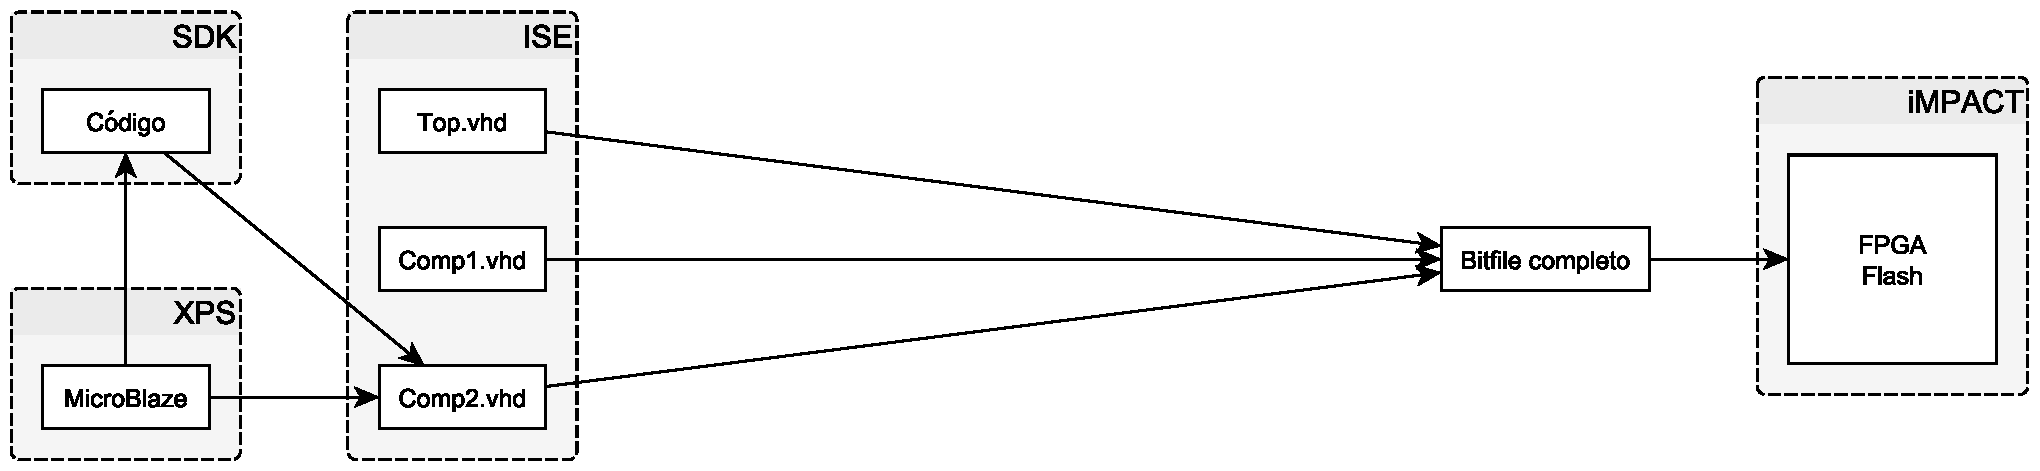
\includegraphics[height=100px]{fig/c3_desenvolvimento/ex1/softwareflow.pdf}
		\caption{Foto ilustrativa do fluxo de ferramentas tradicional. Note que o uso do microcontrolador MicroBlaze é opcional, tornando os primeiros blocos, SDK e XPS, também opcionais.}
		\label{fig:ex1:softwareflow}
	\end{subfigure}\\
	\begin{subfigure}[b]{\textwidth}
		\centering
		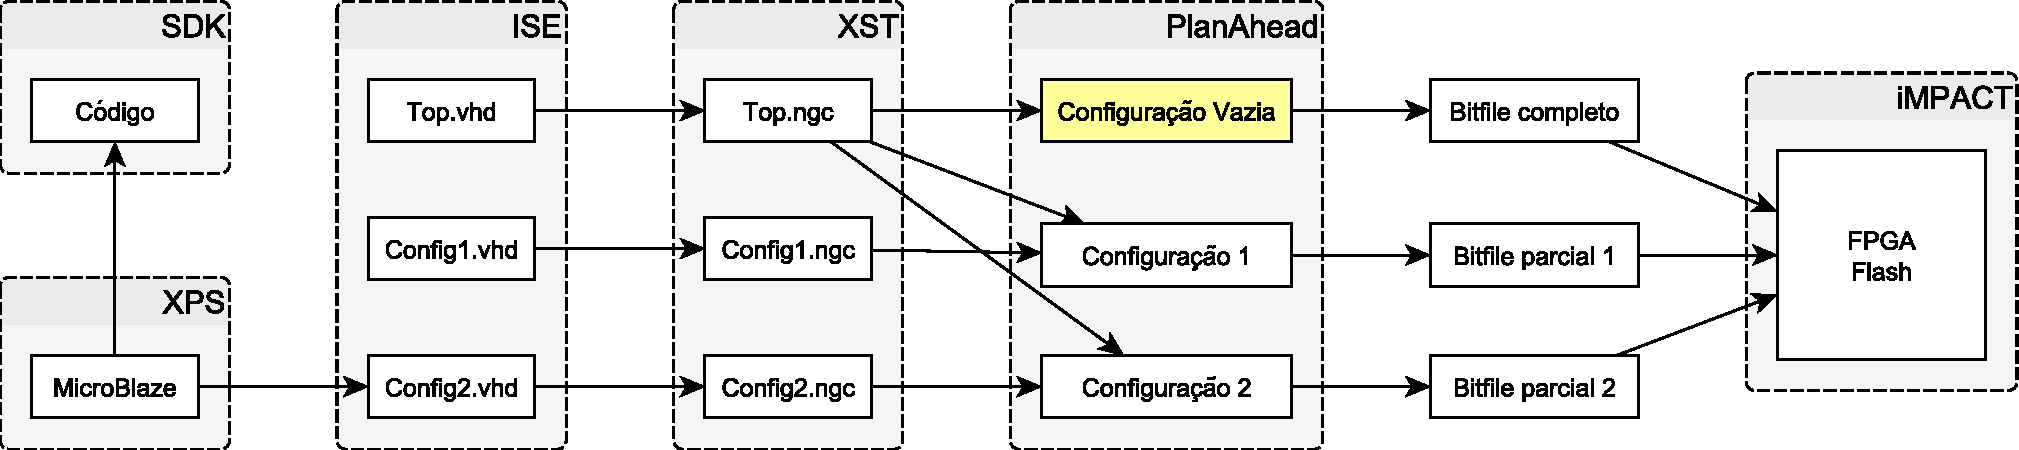
\includegraphics[height=100px]{fig/c3_desenvolvimento/ex1/prsoftwareflow.pdf}
		\caption{Foto ilustrativa do fluxo de ferramentas para a reconfiguração dinâmica. Assim como no caso tradicional, o uso do SDK e do XPS são opcionais. Note que o bloco em amarelo indica a configuração padrão, que será programada inicialmente. A escolha da configuração padrão é arbitrária.}
		\label{fig:ex1:prsoftwareflow}
	\end{subfigure}
	\caption{Comparação dos fluxos de ferramentas. Note que estes fluxos não apresentam as únicas opções de fluxo de ferramentas, mas as que foram utilizadas neste projeto.}
	\label{fig:ex1:softwareflow:comparacao}
\end{figure}

Reconfiguração parcial pede uma síntese utilizando o método \dlq de baixo para cima\drq{} (\textit{bottom-up}), mas uma implementação \dlq de cima para baixo\drq{} (\textit{top-down}) \cite{ug743}, ou seja, a implementação acontece construindo primeiro a interface com o sistema e depois os componentes auxiliares, mas a síntese precisa ser realizada no sentido oposto.
Esta implementação é equivalente a se construir diversos projetos tradicionais com alguma lógica em comum, onde a síntese deve garantir que esta lógica em comum seja implementada da mesma forma para as diferentes configurações \cite{ug702}.

\subsection{Peculiaridades}
O kit de desenvolvimento utilizada apresenta algumas peculiaridades com relação aos kits comuns.
A seguir serão apresentadas algumas destas peculiaridades.

\subsubsection{Relógios}
Diferentemente das FPGAs comuns, a que está presente neste kit contém um relógio diferencial, ou seja, dois sinais compoem tal relógio.
A razão para tal é a presença de circuitos sensíveis a interferência, tais como \textit{transceivers}, que são muito menores em sinais diferenciais.
O kit disponibiliza duas opções de relógio: o SYSCLK e o USER\_CLOCK.
O primeiro possui uma frequência fixa de oscilação de 200 MHz.
O segundo possui uma frequência original de 156,250 MHz, mas pode ser programado através de uma interface I$^2$C para ter frequências entre 10 MHz e 810 MHz.
Por motivos de simplicidade, utilizou-se o SYSCLK.
Para poder se trabalhar com o sinal diferencial, construiu-se, utilizando as ferramentas do ISE, um componente para tratamento do sinal de relógio.
Este componente recebe o sinal diferencial, reduz sua frequência para 20 MHz, que corresponde ao menor valor suportado pelas PLLs da placa, e emite um sinal convencional.

\subsection{Teste}
Para se entender mais a fundo o fluxo de projeto, nada melhor que construir um projeto.
Para isso, implementou-se o sistema esquematizado na figura \ref{fig:ex1:componentes}.
Este sistema contém o \dlq{}Top\drq{} para interfaceamento com a FPGA, o \dlq{}Clocks\drq{} para tratamento do sinal de relógio, a \dlq{}Static\drq{}, que possui um lógica estática para demonstrar que a reconfiguração de uma partição não interfere com outra, e a \dlq{}Dynamic\drq{}, que possui a lógica a ser alterada dinâmicamente.

\begin{figure}[h]
\centering
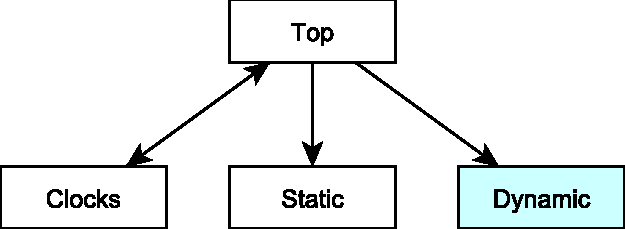
\includegraphics[width=0.5\textwidth]{fig/c3_desenvolvimento/ex1/componentes.pdf}
\caption{Foto ilustrativa do sistema desenvolvido para o teste de validação do experimento 1. Ele é composto por uma parte estática e uma parte dinâmica. O elementos em branco são estáticos e os em azul são dinâmicos.}
\label{fig:ex1:componentes}
\end{figure}

\paragraph{Estrutura de Pastas}
A questão da organização do projeto em pastas bem específicas é sempre bem mencionado na literatura \cite{ug702, ug743, ug744}.
Os manuais recomendam a seguinte estrutura de pastas.
\begin{lstlisting}
Projeto/
  Source/           //codigos-fonte organizados segundo particao
  Implementation/   //contem pastas para cada config. dinamica gerada
  Synth/            //contem pastas com os arquivos .xst e .prj
  Tools/            //ferramentas para automacao da sintese
  PlanAhead/        //pasta para o projeto do PlanAhead
\end{lstlisting}
Esta estrutura de pastas foi obedecida por ajudar a manter o ambiente de desenvolvimento limpo.

\subsubsection{Comportamento}
Como explicado anteriormente, o projeto de um sistema parcialmente reconfigurável pode ser visto como vários projetos completos com partes em comum.
Seguindo essa lógica, dois projetos com comportamentos diferentes foram construídos usando como base a figura \ref{fig:ex1:componentes}.
O comportamento individual de cada módulo ou componente será descrito a seguir.
Este passo está ilustrado no fluxo de ferramentas da figura \ref{fig:ex1:prsoftwareflow} como ISE.

O componente \dlq{}Static\drq{} possui uma entrada para um relógio pulsando a 2 Hz e uma saída para um LED.
Seu comportamento apenas faz com que o LED pisque a uma frequência de 2 Hz, o que permite observar seu funcionamento durante a reconfiguração do componente \dlq{}Dynamic\drq{}.

O componente \dlq{}Dynamic\drq{} possui dois comportamentos distintos.
O primeiro deles é o de um simples contador crescente de 4 bits.
O segundo é uma máquina de estados que alterna os 4 bits de saída entre "1100" e "0011" a cada pulso de relógio.
Este componente possui uma entrada para um relógio pulsando a 1 Hz e uma palavra de 4 bits de saída.
A frequência de operação deste componente foi escolhida para ser a metade da frequência da \dlq{}Static\drq{} para poder ser visualmente comprovado que \dlq{}Static\drq{} não para de funcionar quando \dlq{}Dynamic\drq{} está sendo reconfigurado.

O componente \dlq{}Clocks\drq{} recebe os sinais diferenciais de relógio e o transformam em um sinal comum.
O bloco lógico utilizado para isso foi construído usando ferramentas presentes no ISE.
Uma vez que a ferramenta permitia a construção de um relógio com divisor de frequência, a frequência do relógio da placa, que nesse caso é de 200 MHz, foi reduzida para 20 MHz.

O módulo \dlq{}Top\drq{} instancia os componentes descritos acima e faz a interface dos mesmos com a FPGA.
O componente dinâmico precisa de uma declaração de protótipo para ser instanciado corretamente.
Utilizou-se o código abaixo para esta finalidade.
\begin{lstlisting}[style=customVHDL]
component dynamic
    port ( clk  : in  std_logic;
           leds : out std_logic_vector (3 downto 0));
end component;
\end{lstlisting}
O módulo \dlq{}Top\drq{} possui também um divisor de frequência para reduzir a frequência devolvida por \dlq{}Clocks\drq{} para 1 e 2 Hz.

\subsubsection{Síntese}
Com o comportamento do projeto definido, o próximo passo segundo o fluxo de ferramentas é a síntese.
Este passo é necessário uma vez que o próximo passo, referente ao PlanAhead, não aceita como entrada códigos-fonte.
Os códigos-fonte precisam passar por uma etapa de síntese separada para poderem ser importados no PlanAhead.
Este passo está ilustrado no fluxo de ferramentas da figura \ref{fig:ex1:prsoftwareflow} como XST.

O comando XST recebe tipicamente um \textit{script} contendo o endereço dos códigos-fonte, o nome do arquivo de saída, o tipo do arquivo de saida, o modelo da FPGA utilizada e uma indicação do código-fonte principal.
O comando para iniciar o processo é o seguinte.
\begin{lstlisting}[style=customVHDL]
xst.exe -ifn Top.xst
\end{lstlisting}
O arquivo \dlq{}Top.xst\drq{} contém os seguintes comandos.
\begin{lstlisting}[style=customVHDL]
run
-ifn Top.prj
-ofn Top
-ofmt NGC
-p xc7k325t-2-ffg900
-top top
\end{lstlisting}
O arquivo \dlq{}Top.prj\drq{} contém os endereços dos arquivos, conforme a seguir.
\begin{lstlisting}[style=customVHDL]
vhdl work "../../Sources/static/top.vhd"
vhdl work "../../Sources/static/static.vhd"
vhdl work "../../Sources/static/clocks.vhd"
\end{lstlisting}\

Note que estes comandos e arquivos indicados acima são para síntese dos componentes estáticos.
Uma vez que não existe nenhuma restrição especial para tais componentes, eles podem ser síntetizados para um único arquivo de saída.
O mesmo não pode ser dito para os elementos dinâmicos.
Cada componente dinâmico precisa ser sintetizado em separado para depois ser incluído no projeto através do PlanAhead.

A síntese de componentes dinâmicos precisa ser realizada com um \textit{script} \dlq{}.xst\drq{} ligeiramente diferente.
Como mostrado a seguir, faz-se necessária a inclusão do argumento \dlq{}-iobuf NO\drq{}, que desabilita a inserção de componentes de Entrada/Saída \cite{ug743, ug748}.
\begin{lstlisting}[style=customVHDL]
run
-ifn DynFSM.prj
-ofn DynFSM
-ofmt NGC
-p xc7k325t-2-ffg900
-top dynamic
-iobuf NO
\end{lstlisting}
Note que o arquivo \dlq{}DynFSM.prj\drq{} contém informações sobre o cógigo-fonte do componente dinâmico, como mostrado a seguir.
\begin{lstlisting}[style=customVHDL]
vhdl work "../../Sources/dynamic_fsm/dynamic.vhd"
\end{lstlisting}

Existe também a possibilidade de construção de um \textit{script} para a síntese automática de todos os arquivos.
Utilizou-se aqui uma adaptação do arquivo em linguagem TCL usado pela Xilinx em seus manuais \cite{ug702, ug743, ug744}.
A única coisa que se faz neste \textit{script} é a construção dinâmica dos comandos com base em listas de arquivos pré-informados.

\subsubsection{PlanAhead}
Com os arquivos síntetisados, pode-se começar a etapa referente ao PlanAhead.
Nela, importaremos os arquivos da etapa anterior, criaremos a partição reconfigurável, mapearemos esta partição no dispositivo, criaremos configurações alternativas, promoremos tais configurações e geraremos os \textit{bitfiles} para a programação do dispositivo.
Note que é preciso uma licença do ISE que permita o uso do PlanAhead e de reconfiguração parcial.

O primeiro passo necessário no PlanAhead é a criação do projeto.
Para isso, após a abertura do programa, clica-se no ícone superior esquerdo mostrado na figura \ref{fig:ex1:planahead}, onde se lê \dlq{}Create New Project\drq{}.
Na janela que aparece, indicamos o nome do projeto e seu caminho, lembrando que foi criada uma pasta anteriormente especificamente para conter este projeto.
Indicamos também que o projeto é do tipo \dlq{}\textit{Post-synthesis Project}\drq{} e que desejamos habilitar a reconfiguração parcial, indicamos quais \textit{netlists} compõe o comportamento do projeto e qual corresponde ao arquivo principal, qual é o arquivo de restrições (\textit{constrains}) e qual é o modelo da FPGA.

\begin{figure}[h]
\centering
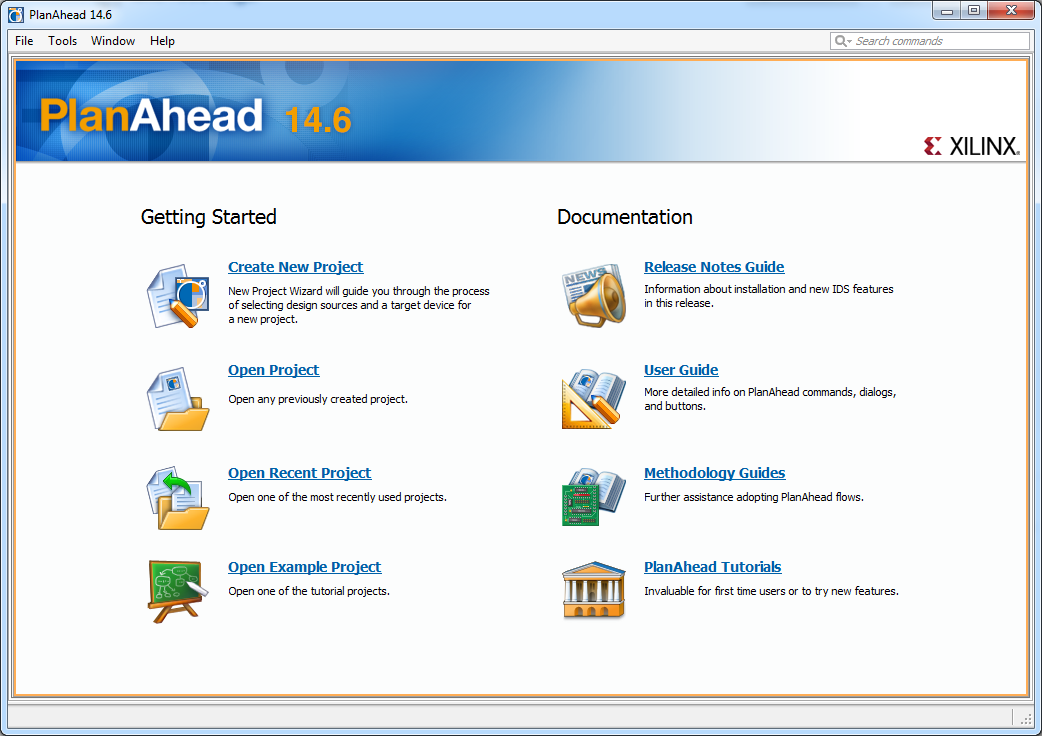
\includegraphics[width=0.9\textwidth]{fig/c3_desenvolvimento/ex1/PlanAhead}
\caption{Imagem do PlanAhead logo que aberto.}
\label{fig:ex1:planahead}
\end{figure}

Após a criação do projeto, carregam-se os arquivos sintetizados abrindo \dlq{}\textit{Open Synthesized Design}\drq{}, mostrado na figura \ref{fig:ex1:planahead_open_synthesized_design}.
Duas janelas de avisos aparecem, informando que existe uma partição não implementada e aviso sobre alguns pinos.

\begin{figure}[h]
\centering
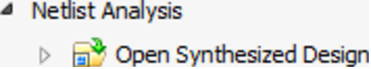
\includegraphics[width=173px]{fig/c3_desenvolvimento/ex1/planahead_open_synthesized_design}
\caption{Imagem do menu \dlq{}\textit{Open Synthesized Design}\drq{}.}
\label{fig:ex1:planahead_open_synthesized_design}
\end{figure}


Pode-se agora definir a partição que armazenará o componente dinâmico.
Isso é feito através do painel \dlq{}\textit{Netlist}\drq{}, selecionando a opção \dlq{}\textit{Set Partition}\drq{} do menu que aparece ao se clicar em \dlq{}dynamic\_i\drq{} com o botão direito.
Na janela que aparece, selecionamos a opção referente à partição reconfigurável, nomeamos o módulo reconfigurável de acordo com o componente que será carregado e indicamos o arquivo que corresponde ao arquivo sintetizado do componente reconfigurável.
Não é necessário informar restrições, visto que o componente, seguindo recomendações, não acessa os pinos de entrada e saída diretamente.
Note ainda que é recomendado que o primeiro módulo a ser incluído seja o mais complexo e sucetível a falhas, permitindo que erros e falhas na definição da região a seguir sejam identificados mais cedo.

Precisa-se definir também uma região para a partição recém definida.
Isto pode ser feito pelo mesmo painel \dlq{}\textit{Netlist}\drq{}, selecionando a opção \dlq{}\textit{Set Pblock Size}\drq{} do menu que aparece ao se clicar em \dlq{}dynamic\_i\drq{} com o botão direito.
Nesse momento, precisa-se selecionar na aba \dlq{}\textit{Device}\drq{} uma região do dispositivo que contenha uma quantidade de recursos maior que a requerida pelo projeto.
Note que o processo de escolha dessa região não é bem definido, o que abre espaço para diversos erros de alocação.
Para testar se a região foi bem alocada, abre-se a aba \dlq{}\textit{Design Runs}\drq{} do painel inferior, clica-se com o botão direito na única configuração disponível no momento e seleciona-se \dlq{}\textit{Run Launch}\drq{}.
Este processo pode demorar.
Em tentativas subsequentes, seleciona-se a opção de recomeçar todo o processo do zero, evitando erros gerados nos estágios iniciais.
Uma região possível, que foi utilizada nesse projeto, foi a que contém as células (\textit{slice}) de X80Y244 a X139Y205.
Os nomes das células ficam visíveis através da ampliação do dispositivo.

Uma vez terminado o \dlq{}\textit{Design Run}\drq{}, adiciona-se duas novas possibilidades de módulos reconfiguráveis para esta partição: um com comportamento definido e outro vazia.
Para isso, clica-se em \dlq{}\textit{Synthesized Design}\drq{} novamente e seleciona-se a opção \dlq{}\textit{Add reconfigurable module}\drq{} do menu que aparece ao se clicar em \dlq{}dynamic\_i\drq{} no painel \dlq{}\textit{Netlist}\drq{} com o botão direito.
O processo é o mesmo da definição da partição, sendo a única mudança na seleção do arquivo sintetizado e do nome do módulo.
Um módulo vazio pode ser criado usando esta mesma opção, mas selecionando a opção que indica a inclusão de uma \textit{blackbox} sem o uso de uma \textit{netlist}.

Com as possibilidades de módulos reconfiguráveis definidas, pode-se construir várias configurações.
Isso é feito através do clique com botão direito na \dlq{}\textit{Design Runs}\drq{} do painel inferior e selecionando-se a opção \dlq{}\textit{Create Runs...}\drq{}.
A janela que abre possui um painel chamado \dlq{}\textit{Create Implementation Runs}\drq{}.
Nesse painel, na coluna \dlq{}\textit{Partition Action}\drq{}, define-se, na coluna \dlq{}\textit{Module Variant}\drq{} da nova janela que aparece, o módulo desejado.
Voltando para a primeira janela, clica-se em \dlq{}\textit{More}\drq{} para adicionar a última configuração desejada.
Em seguida, as duas novas configurações serão criadas através de \dlq{}\textit{Design Runs}\drq{}.
É necessário promover neste momento a primeira configuração implementada.
O processo de promoção será comentado a seguir.
Note que os avisos que aparecerem podem ser ignorados.

Ao final dos \dlq{}\textit{Design Runs}\drq{}, recomenda-se fazer a verificação das configurações através do painel \dlq{}\textit{Configurations}\drq{}.
Clicando-se com o botão direito, encontra-se a opção \dlq{}\textit{Verify Configuration...}\drq{}, que faz com que uma janela seja aberta.
Selecionado-se todos os itens e clicando em \dlq{}\textit{OK}\drq{}, a verificação se inicia.
Nenhum erro deve ser encontrado.

Devemos agora promover as configurações.
No menu de quando se clica com o botão direito sobre as configurações já existentes do painel \dlq{}\textit{Configurations}\drq{}, seleciona-se \dlq{}\textit{Promote Configuration...}\drq{}.
A promoção de uma configuração é o equivalente a sua exportação \cite{ug748}.
Promover a primeira configuração antes de implementar novas contribui para manter a parte estática, compartilhada, igual em todas as configurações, uma vez que elas não mais são sintetizadas e sim importadas.

O último passo necessário para a criação dos \textit{bitfiles} é o \dlq{}\textit{Generate Bitstream}\drq{}, localizado no menu a esquerda.
Este passo recebe o resultado das sínteses e implementações e transforma-os em \textit{bitfiles}.
Esta etapa precisa ser realizada com cada uma das configurações realizadas, ou alguma delas não terá seus \textit{bitfiles} gerados.
Tais \textit{bitfiles} podem ser encontrados na pasta do projeto, dentro das pastas com nome de cada configuração que ficam dentro de da pasta *.runs.
Existem dois arquivos \textit{bitfile} dentro de cada pasta, um maior, que contém a configuração completa, e outro menor que possui a configuração parcial.

\subsubsection{iMPACT}
Com os \textit{bitfiles} em mãos, usa-se-os para programar a FPGA através auxilio da ferramenta iMPACT. 
A primeira coisa a se fazer após abrir o programa é permitir que o sistema automaticamente crie um projeto.
Na janela que se abre, escolhe-se a opção \dlq{}\textit{Automatically connect to a cable and identify Boundary-Scan chain}\drq{} do item \dlq{}\textit{Configure devices using Boundary-Scan (JTAG)}\drq{}.
Quando pergunta-se se deseja-se atribuir uma nova configuração, pode-se clicar que sim e escolher um arquivo binário completo gerado na etapa anterior.
Normalmente escolhe-se a configuração vazia como configuração inicial para poupar energia.

Quando a configuração for completamente transmitida e implementada, observa-se que um LED está piscando com uma frequência de 2 Hz e todos os outros (acionados) estão acesos.
Isto acontece uma vez que o sitema atribui sinal ativo para os elementos desconectados.

Para realizar a reconfiguração parcial dinâmica, clica-se com o botão direito no símbolo do dispositivo que aparece no iMPACT e seleciona-se a opção \dlq{}\textit{Assign New Configuration File...}\drq{}.
Procura-se então pelos arquivos binários parciais localizados na pasta \textit{PlanAhead > PlanAhead.runs >} \dlq{}nome da configuração\drq{}.
Este arquivo possui \dlq{}partial\drq{} em seu nome, o que o diferencia do arquivo binário completo.
Note que utilizar os arquivos binários completos não gera erro, mas constitui reconfiguração total, não parcial.
Após a seleção da configuração desejada, o último passo necessário é a programação, que pode ser realizada clicando-se com o botão direito no dispositivo e selecionando-se a opção \dlq{}\textit{Program}\drq{}.

\subsection{Possíveis Erros}
\paragraph{Erros no código-fonte} Este é um dos erros mais comuns.
A melhor forma de previní-lo é através da construção dos diversos comportamentos/configurações individuais utilizando o ISE.
Para acelerar o processo, realiza-se apenas a síntese.

\paragraph{Erros na alocação de partições}
Um erro bastante comum que aparece no PlanAhead é o de erro de alocação\footnote{\textit{AR\# 53290: Partial Reconfiguration - 7 series device layout of tiles (CLB, DSP, BRAM, INT) and a shared clocking structure of vertical clock spines between interconnect (routing) tiles}. Disponível em \url{http://www.xilinx.com/support/answers/53290.htm}}.
Existem duas possíveis formas de corrigí-lo: modificando-se o arquivo de restrições UCF ou alterando a região da partição.
A primeira forma, que ajuda a garantir que todos os recursos reconfiguráveis estão incluidas na região da partição, é a inclusão de \dlq{}INCLUSIVE=ROUTE\drq{} na linha que contém \dlq{}INST "dynamic\_i" AREA\_GROUP = "pblock\_dynamic\_i"\drq{}.
A segunda forma é simplemente mudando a posição da região da partição para a direita, para a esquerda ou sua largura, de acordo com a mensagem de erro retornada.
Esta método não é determinístico e pode ser necessárias várias tentativas antes de se conseguir uma partição mapeável. 

\paragraph{Esquecer de promover a partição}
A promoção da primeira configuração antes de se implementar as seguintes contribui para a implementação de configurações compatíveis.
Esquecer de promover esta partição pode fazer com que erros sejam gerados na etapa de verificação das partições.

\paragraph{O PlanAhead pode travar enquanto implementando uma configuração}
Apesar de mais raro, o PlanAhead pode travar quando implementando uma configuração.
A melhor solução é o reinício do computador, visto que o programa bloqueia alguns arquivos durante a implementação e não os desbloqueia quando fechado forçadamente.

\paragraph{Erros na detecção da placa}
Note que algum programa aberto pode interferir com a varredura realizada pelo iMPACT, fazendo-a falhar.
Para prevenir este erro, deve-se fechar o XPS, o SDK e qualquer outro programa que possa se utilizar das interfaces USB.
Note ainda que a placa deve estar ligada para poder ser detectada.

\subsection{Conclusão}
O processo de desenvolvimento de partições reconfiguráveis e sua programação foi explorado com sucesso.
Observou-se os pontos críticos do desenvolvimento e o fluxo mais adequado para a construção deste tipo de projeto.

\section{Experimento 2 - Teste de Memórias}
Seguindo o raciocínio apresentado no início do capítulo, o próximo passo natural no desenvolvimento deste projeto é o entendimento do funcionamento das memórias.
Esta etapa abre caminho para que se armazene os \textit{bitfiles} de configurações parciais em uma memória embarcada, removendo a necessidade do computador para tal.

\subsection{Tipos de Mémoria}

No kit utilizado existem vários tipos de memórias que poderiam ser usados, cada um com suas peculiaridades \cite{ug810}.
Este experimento foi dedicado à compreenção do funcionamento dos diversos tipos de memórias e à escolha da solução mais adequada.

\subsubsection{Memória \textit{Block RAM}}
A memória do tipo \textit{Block RAM} é construída usando-se os blocos de memória RAM restantes da FPGA.
Esta memória consegue alcançar velocidades de leitura na ordem de várias centenas de hertz, mas possui uma capacidade de armazenamento bem reduzida, de apenas 445 blocos de 36 Kb para este kit, totalizando um máximo de aproximadamente 2 MB \cite{ug473, wp377}.
Note que a configuração total da FPGA necessita de aproximadamente 11 MB, ou exatamente 91.548.896 bits, para sua programação total \cite{ug470}.
Pode-se programá-la através do iMPACT, dentre outras formas \footnote{\textit{Memory Initialization Methods}, escrito por Jim Wu em 31 de dezembro de 2011. Dísponível em \url{http://myfpgablog.blogspot.com.br/2011/12/memory-initialization-methods.html}}.

\subsubsection{Memória \textit{Distributed RAM}}
A memória \textit{Distributed RAM} é construida utilizando-se das LUTs disponíveis nas célula lógicas \cite{ug473, wp377}.
Também são muito rápidas, apesar de síncronas, e também possuem pouca capacidade de armazenamento.
Pode-se programá-la através do iMPACT, dentre outras formas.

\subsubsection{Memória \textit{Linear BPI Flash}}
A memória \textit{Linear BPI Flash} disponibiliza 128 Mb de memória não-volátil \cite{ug810}, acessadas em palavras de 16 bits.
Apesar disso, sua velocidade de leitura máxima é de 33 MHz.
Convertendo tal velocidade para a leitura de 32 bits, tem-se uma velocidade de leitura de aproximadamente 16 MHz.
Pode-se programá-la através do iMPACT.

\subsubsection{Memória \textit{SPI Flash}}
A memória SPI Flash é diferente na sua forma de acesso, que acontece através da interface SPI.
Esta memória fornece 128 Mb de memória não volátil \cite{ug810}.
Ela aceita três modos de operação, x1, x2 e x4, que corresponde a largura da palavra lida/escrita a cada pulso de relógio \cite{N25Q128}.
A frequência de operação é de no máximo 50 MHz \cite{xapp586}.
Pode-se programá-la através do iMPACT.

\subsubsection{Cartão de Memória SD}
O cartão de memória SD dá acesso a uma memória não-volátil de tamanho arbitrário.
Esta interface permite o uso de cartões de alto desempenho, lendo palavras de 4 bits a frequências de até 50 MHz \cite{ug810}.
A limitação desta interface é a dificuldade de leitura e escrita devido ao sistema de arquivos inerente ao cartão.
Note que também não existe a possibilidade de programação do cartão através do iMPACT, o que resolveria o problema do sistema de arquivos.

\paragraph{\textit{CompactFlash} e o \textit{System ACE}}
\textit{SystemAce} é um sistema que permite a programação de FPGAs e memórias voláteis a partir de um cartão \textit{CompactFlash} \cite{ds080, ds583}.
Este é bem robusto e popular em séries que possuem um leitor deste tipo de cartão.

\subsubsection{Memória DDR3}
A memória DDR3 é uma memória volátil com 1 GB de capacidade de armazenamento e possui uma frequência de operação da ordem dos 800 MHz \cite{MT8JTF12864HZ}.
Só pode ser programada apenas em tempo de execução, fazendo-se necessário o uso de um \textit{bootloader}.

\subsection{Teste}
Notou-se no primeiro experimento que os \textit{bitfiles} parciais gerados possuem 645 KB, totalizando 1935 KB, ou 1,89 MB.
Com isso o uso das memórias que se utilizam de recursos internos da FPGA fica comprometido.
Caso se escolha esta opção, apenas os \textit{bitfiles} parciais poderiam ser armazenados, necessitando da ajuda do computador para a programação inicial.
Este típo de memória é mais útil como memória de dados e de programa em microcontroladores embarcados na FPGA, devido a sua altíssima velocidade de acesso e capacidade de acesso de vários canais em paralelo.

Observa-se que a interface de reprogramação dinâmica, ICAPE2, opera a uma frequência de até 100 MHz e pode receber palavras de até 32 bits, ou seja, 3200 Mb/s.
Por causa disso, todas as interfaces não-voláteis apresentadas acima acabariam por ser o gargalo do tempo da programação.
Uma solução é a implementação de um sistema que carregue as informações de uma memória não-volátil, tanto a Linear Flash quanto a SPI Flash seriam suficientes, para a memória DDR3 em um momento inicial, e depois permita que a memória DDR3 seja acessada para a reconfiguração dinâmica.
A forma mais fácil de implementar tal funcionalidade é através do uso de um microcontrolador MicroBlaze funcionando como \textit{bootloader}.

Antes de implementar o \textit{bootloader}, precisamos entender como funcionam as memórias do escolhidas.
Este teste, então, tem por objetivo entender o fluxo de projeto para o uso do MicroBlaze, o funcionamento deste microcontrolador e as formas corretas de se acessar as memórias do sistema.

\subsubsection{Fluxo de Projeto}
O procedimento para a construção de um projeto com MicroBlaze segue o fluxo descrito na figura \ref{fig:ex1:softwareflow}, no que diz respeito ao XPS e ao SDK.
A figura \ref{fig:ex2:softwareflow} apresenta o fluxo de ferramentas para este caso específico.
Em outras palavras, o fluxo espera que primeiro se desenvolva o microprocessador com todos os seus periféricos para depois se desenvolver o programa que será embarcado.
Tanto o programa quando o processador gerarão arquivos binários que serão carregados pelo iMPACT através do SDK.

\begin{figure}[htp]
\centering
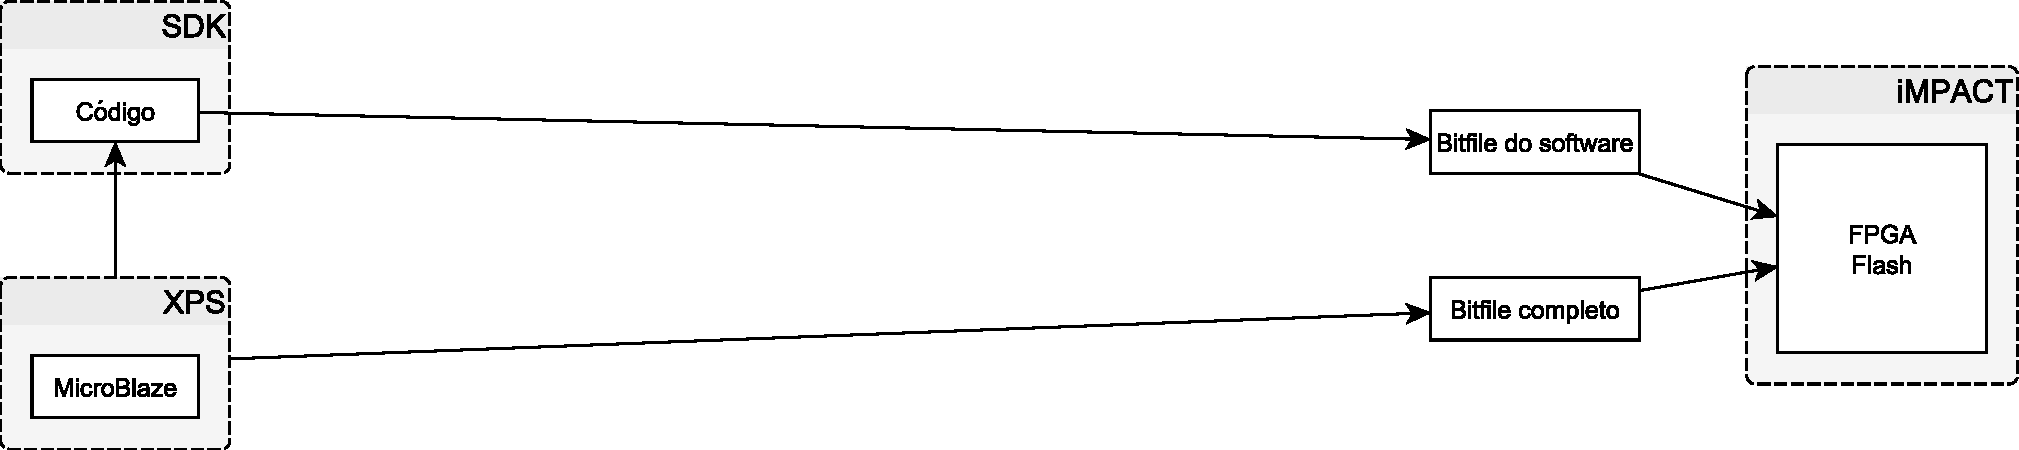
\includegraphics[height=100px]{fig/c3_desenvolvimento/ex2/softwareflow.pdf}
\caption{Foto ilustrativa do fluxo de ferramentas para o desenvolvimento de sistemas com MicroBlaze, extraído de \cite{ug081}.}
\label{fig:ex2:softwareflow}
\end{figure}

\subsubsection{MicroBlaze}
O MicroBlaze é um microprocessador otimizado para implementação em FPGAs da Xilinx \cite{ug081}.
Ele possui 32 registrados genéricos de 32 bits, instruções de 32 bits e endereços de 32 bits.
Seu \textit{pipeline} possui 3 ou 5 estágios e é construido em torno da arquitetura Harvard, como pode ser observado na figura \ref{fig:ex3:microblazecore}.
Todas as outras configurações, tais como o uso de \textit{Big Endian} ou \textit{Little Endian}, por exemplo, são opcionais \cite{ug081}.

\begin{figure}[h]
\centering
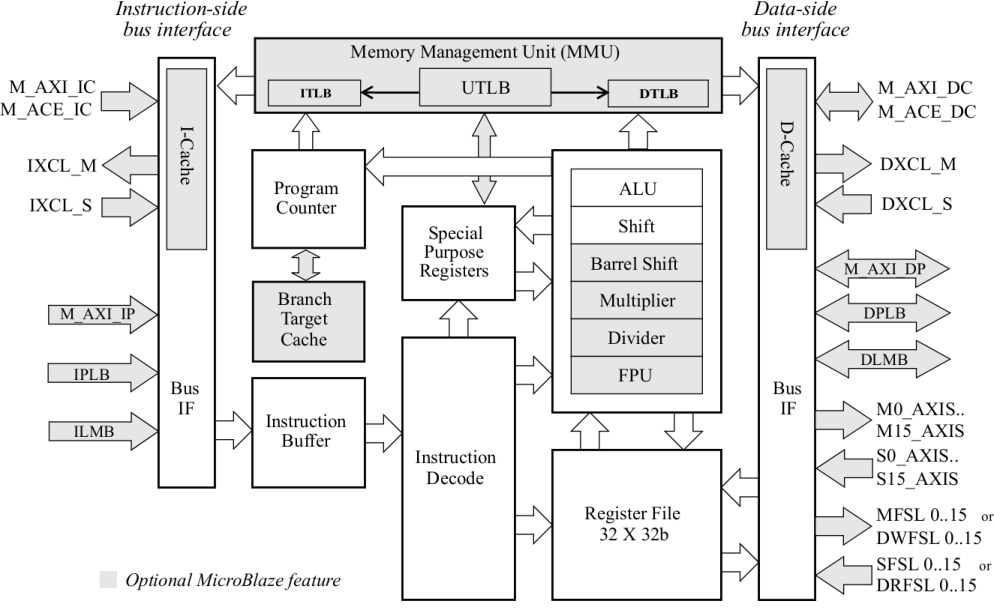
\includegraphics[width=0.9\textwidth]{fig/c3_desenvolvimento/ex2/MicroBlaze_Core.pdf}
\caption{Diagrama de blocos do MicroBlaze.}
\label{fig:ex3:microblazecore}
\end{figure}

O MicroBlaze permite o uso de diversas interfaces para comunicação com seus diversos periféricos, dentre elas a PLB, a LMB, a AXI e a ACE \cite{ug081}.
A interface mais atual suportada, e que foi utilizada neste experimento, é a Advanced eXtensible Interface 4 (AXI4) \cite{ug081, ug761}.
A AXI4 é uma interface mapeada em memória que oferece produtividade, flexibilidade e disponibilidade.
Ela possui três tipos de interfaces, a AXI4, a AXI4-Lite e a AXI4-Stream, onde as duas primeiras são compostam de 5 canais de comunicação: de leitura de endereço, de escrita de endereço, de leitura de dados, de escrita de dados e de escrita de resposta.

\subsubsection{XPS}
Para começar, deve-se abrir o programa e criar um novo projeto usando o \textit{Base System Builder} (BSB), opção que corresponde ao item superior esquerdo do menu da tela inicial.
Na janela que aparece, escolheu-se a placa de desenvolvimento Kintex-7 KC705 \textit{Evaluation Platform}, \textit{Board Revision} C, e a opção de um só processador no sistema, para simplificar o projeto.
Dando prosseguimento, escolheu-se os periféricos desejados segundo a figura \ref{fig:ex2:bsb_prerifericos} e o tamanho das memórias local, de intrução e de dados, quiça 64 KB.
Modificou-se ainda, como pode-se ver na figura \ref{fig:ex2:bsb_prerifericos}, o \textit{Baud Rate} da interface UART para 115200 bits/s.

\begin{figure}[htp]
\centering
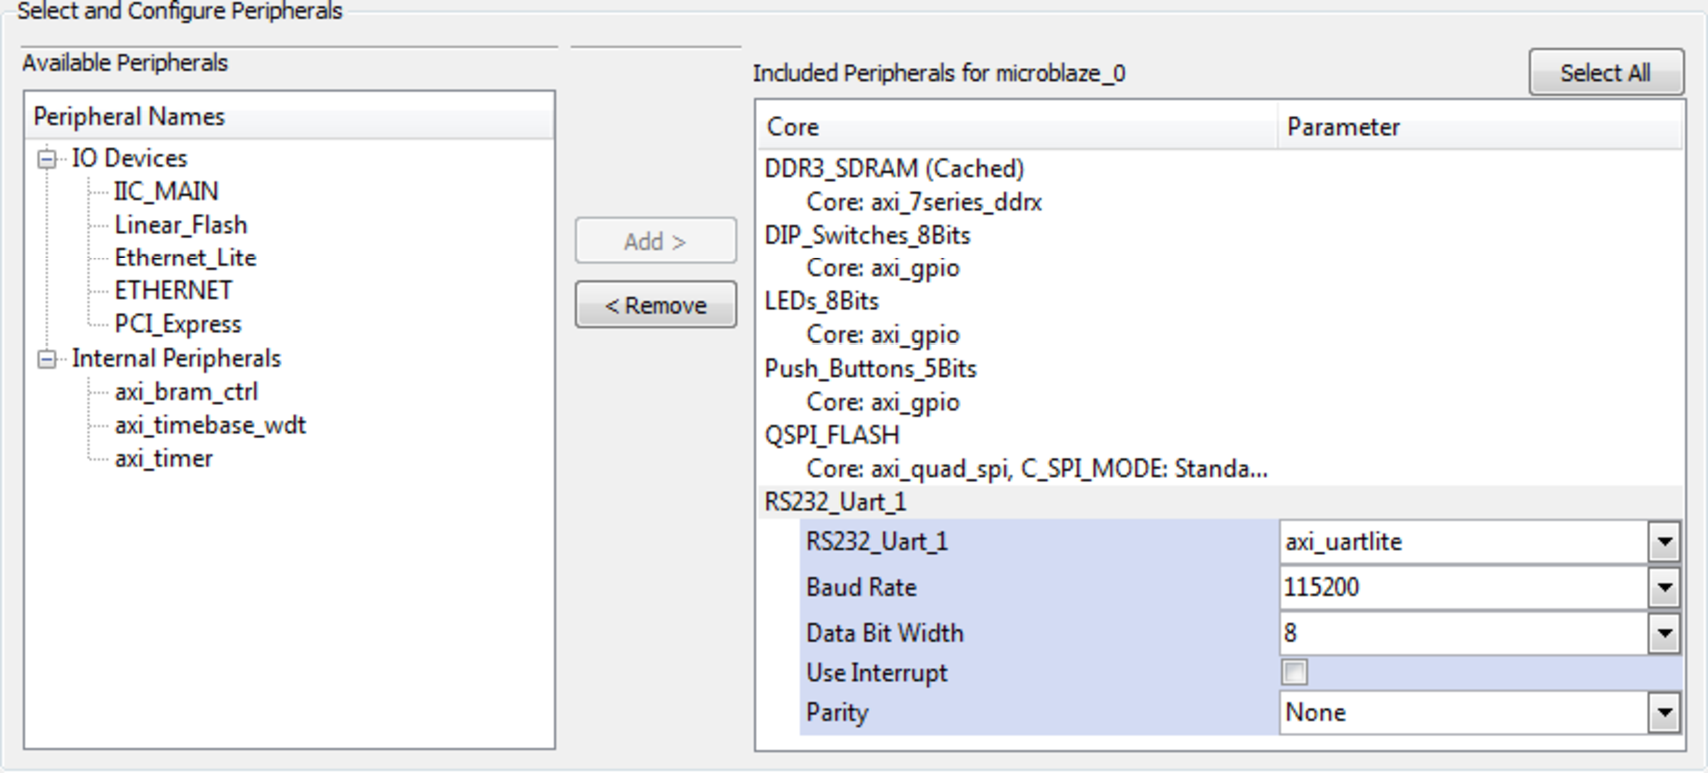
\includegraphics[width=0.75\textwidth]{fig/c3_desenvolvimento/ex2/BSB_AXI_flow.pdf}
\caption{Escolha dos periféricos no BSB do XPS.}
\label{fig:ex2:bsb_prerifericos}
\end{figure}

Antes de concluir o a construção do sistema, precisa-se ajustar os tamanhos das memórias e seus endereços, de forma que estes novos tamanhos possam ser corretamente acessados.
Isto pode ser feito na aba \textit{Addresses} do painel \textit{System Assembly View}.
Muda-se então o tamanho da memória SPI Flash para 128M, seu endereço base para 0x80000000, o tamanho da memória DDR3 para 1G e seu endereço base para 0xC0000000, conforme a figura \ref{fig:ex2:xps_enderecos}.
Note que o endereço-base da memória SPI Flash tem como única restrição de os 28 bits menos significativos iguais a zero e que o endereço-base da memória DDR3 tem esta mesma restrição para os 30 bits menos significativos.
Estas restrições são devido aos tamanhos das memórias e o alinhamento dos espaços de dados na memória.

\begin{figure}[htp]
\centering
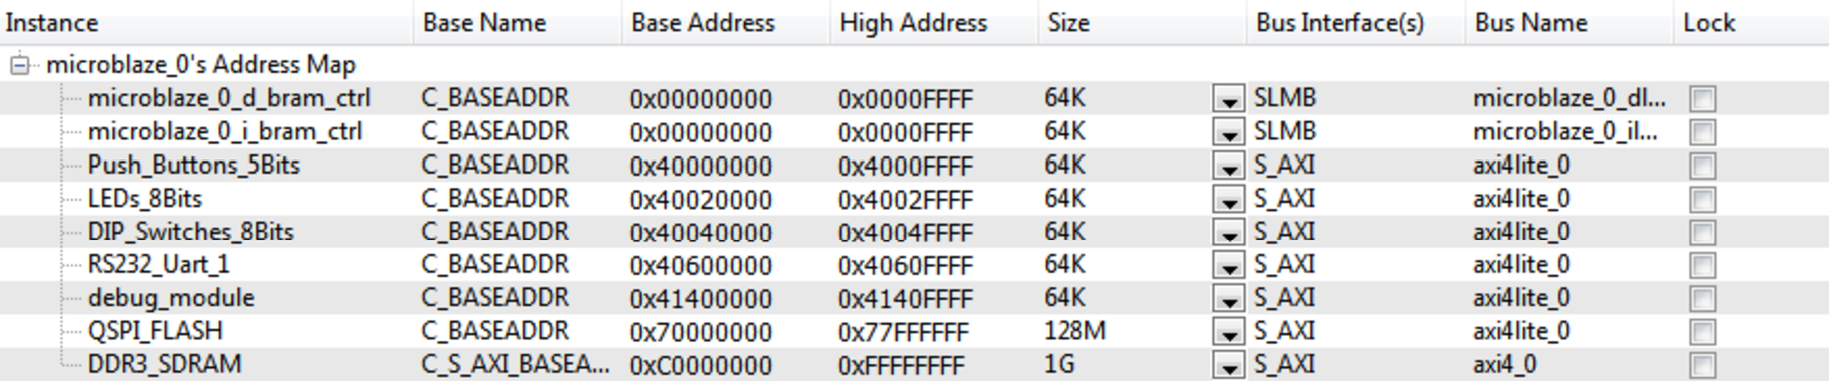
\includegraphics[width=0.7\textwidth]{fig/c3_desenvolvimento/ex2/xps_address.pdf}
\caption{Aba \textit{Addresses} do \textit{System Assembly View} indicando os ajustes dos endereços e tamanhos das memórias.}
\label{fig:ex2:xps_enderecos}
\end{figure}

Precisa-se agora modificar as posições de memória cobertas pela memória \textit{cache}.
Isto é feito clicando-se duas vezes sobre \dlq{}microblaze\_0\drq{} na aba \dlq{}\textit{Bus Interfaces}\drq{} do painel \dlq{}\textit{System Assembly View}\drq{}.
Na janela que se abre, clica-se  \dlq{}\textit{Next}\drq{} 3 vezes para chegar página sobre \textit{caches}.
Modifique os endereços da primeira coluna para 0xc0000000 e 0xffffffff e os da segunda para 0x80000000 e 0xffffffff, indicando que a memória de instruções pode acessar apenas os endereços da memória DDR3, mas que a memória de dados pode acessar toda a faixa de endereços entre 0x80000000 e 0xffffffff, que engloba as memórias SPI Flash e DDR3.
Apenas os endereços contidos neste intervalo da memória de dados podem ser escritos.
Note que o sistema reserva para uso próprio os primeiros 64K endereços das memórias, que correspondem às posições com finais entre 0x0000 a 0x3fff.
A tentativa de uso destes endereços comprometerá o correto funcionamento do sistema.

O projeto pode ser sintetizado através do botão \dlq{}\textit{Generate Netlist}\drq{} localizado no menu a esquerda e no menu \dlq{}\textit{Hardware}\drq{} da barra de menus.
Este processo é demorado.
Quando terminado, pode-se exportar o projeto através do botão \dlq{}\textit{Export Design}\drq{} para abrir o SDK com as informações deste processador.
Na janela que aparecer, marque \dlq{}\textit{Include bitstream and BMM file}\drq{} e clique em \dlq{}\textit{Export \& Launch SDK}\drq{}.
Após a implementação do arquivo binário, a ferramenta SDK será aberta.

\subsubsection{SDK}
Quando a janela do SDK aparecer, ela perguntará onde se quer colocar o \textit{workspace}.
Uma boa opção é a pasta SDK criada dentro da pasta do projeto do sistema durante sua exportação, apesar desta escolha ser completamente arbitrária.
Escolhida a pasta, o ambiente de trabalho é aberto.

Começa-se o processo criando um projeto do tipo \dlq{}\textit{Board Support Package}\drq{}.
Este projeto compila automaticamente os drivers disponíveis para o projeto segundo as características do microcontrolador.
Em seguida, pode-se criar os projetos dos \textit{softwares} que irão embarcados.
Para isto, cria-se um projeto do tipo \dlq{}\textit{Application Project}\drq{}.
Na janela que se abre, nomeie o projeto e selecione a \dlq{}\textit{Board Support Package}\drq{} no \textit{dropdown} do item \dlq{}\textit{Board Support Package}\drq{}.
Na página seguinte, escolhe-se \dlq{}\textit{Empty Project}\drq{}.

Adiciona-se arquivos ao projeto tanto arrastando os códigos para ele quanto selecionando a opção \dlq{}\textit{New/Source File}\drq{} do menu que aparece quando se clica no projeto com o botão direito.
Note que o acesso a memória é feito simplesmente dereferenciando um ponteiro para a posição de memória desejada.
A escrita é feita do mesmo modo.
Encontra-se emanexo códigos-exemplo para o teste das memórias DDR3 e SPI Flash.

Antes de executar o programa, é interessante habilitar a opção de debugação.
Isto é feito através do menu \dlq{}\textit{Run}\drq{}, na opção \dlq{}\textit{Run Configurations...}\drq{}.
Na janela que aparece, na aba \dlq{}\textit{STDIO Connection}\drq{}, habilita-se a conexão do STDIO com o console e modifica-se o \dlq{}\textit{Baud Rate}\drq{} para 115200.
Clica-se então em \dlq{}\textit{Apply}\drq{} e em seguida \dlq{}\textit{Close}\drq{}.

A programação do FPGA pode ser feita através do menu \dlq{}\textit{Xilinx Tools}\drq{}, na opção \dlq{}\textit{Program FPGA}\drq{}.
Na janela que se abre, é padrão que as informações já estejam pré-preenchidas, mas caso isto não aconteça, procura-se pelos arquivos \dlq{}system.bit\drq{} e \dlq{}system\_bd.bmm\drq{} na pasta \dlq{}\textit{implementations}\drq{} na raíz do projeto do processador.
Clica-se em \dlq{}\textit{Program}\drq{} para inciar a programação.

Para se transferir o programa criado com o auxílio do SDK, seleciona-se o projeto deste programa, clica-se com o botão direito, seleciona-se o submenu \dlq{}\textit{Run As...}\drq{} e escolhe-se a opção \dlq{}\textit{1 Launch on Hardware (GDB)}\drq{}.
No caso dos códigos-exemplo, algumas informações são imprimidas no console caso tudo tenha ocorrido confome o esperado.

\subsection{Conclusão}
Conclui-se assim o experimento para o teste de programação das memórias.
Notou-se que existe muita pouca literatura no assunto, forçando o programador a fazer uso dos forúns de discussão e conhecimentos gerais de programação embarcada.
Apesar disso, o objetivo do experimento, quiça conseguir ler/escrever de/em endereços das memória DDR3 e SPI Flash específicos, foi atingido com sucesso.

\section{Experimento 3 - Teste do \textit{Bootloader}}
O \textit{bootloader}, como mencionado acima, é um sistema que carrega as informações de uma memória lenta, a SPI Flash foi escolhida, para uma memória rápida, a memória DDR3.
Usou-se um microcontrolador MicroBlaze com interfaces para as memórias SPI Flash e DDR3.
O experimento 2 foi dedicado a aprender a utilizar estas memórias.
Neste experimento, espera-se entender como é formado o arquivo binário para assim carregá-lo e interpretá-lo enquanto o transferindo para a memória DDR3.

Utilizará-se também o GPIO, que dá acesso aos pinos da placa, visto que é interessante que este subsistema possa sinalizar para os demais que o carregamento foi completado e informar algumas informações dos elementos transferidos, tais como tamanhos e posições iniciais.

\begin{figure}[htp]
\centering
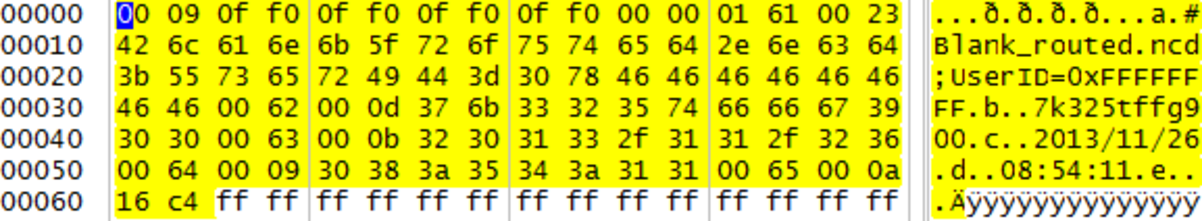
\includegraphics[width=0.8\textwidth]{fig/c3_desenvolvimento/ex3/hex_blank.pdf}
\caption{Cabeçalho do arquivo binário gerado no primeiro experimento para a configuração vazia.}
\label{fig:ex3:hex_blank}
\end{figure}

\subsection{Arquivo Binário}
O arquivo binário é formado por três partes: um cabeçalho, uma palavra para sincronia e a configuração propriamente dita \cite{ug470, xapp583}.
O cabeçalho é formado por chaves e tamanhos, indicando diversos campos deste.
Na tabela \ref{tab:ex3:hex_blank} pode-se observar os tamanhos e campos apresentados na figura \ref{fig:ex3:hex_blank}.
A figura \ref{fig:ex3:hex_blank} possui os primeiros 112 bytes, dos quais os primeiros 98 estão selecionados, da configuração parcial vazia construida no experimento 1.
O primeiro conjunto tamanho/chave indica, através da sequência de de palavras 0x0f, que a configuração é válida.
Se estas palavras fossem 0x00 indicariam que a configuração não é mais válida, e se contivessem 0xff indicariam que a configuração está vazia.

O cabeçalho descrito na tabela \ref{tab:ex3:hex_blank} contém pelo menos duas informações muito interessantes: o identificador do dispositivo alvo, que permite verificar a compatibilidade entre a configuração e o dispositivo que a está recebendo, e o tamanho da configuração, que permite que ela seja carregada de forma dinâmica sem necessidade de mais informações.

\begin{table}[htp]
\centering
\begin{tabular}{cp{4cm}p{7.5cm}}
Tamanho & Chave & Significado\\ \hline
2 bytes & 9 (0x00 09) & Tamanho em bytes do próximo campo \\ \hline
9 bytes & 0x0f f0 0f f0 0f f0 0f f0 00 & Indica que a configuração a seguir é válida. \\ \hline
2 bytes & 1 (0x00 01) & Tamanho em bytes do próximo campo\\ \hline
1 byte & "a" (0x61) & Indica que os próximos campos conterão informações sobre o projeto e sobre a configuração. \\ \hline
2 bytes & 35 (0x00 23) & Tamanho em bytes do próximo campo \\ \hline
35 bytes & Blank\_routed.ncd;\qquad UserID=0xFFFFFFFF & Apresenta o nome do \textit{netlist} e o identificador do usuário. 0x00 ao final indica o final da string. \\ \hline
1 byte & "b" (0x62) & Indica que o próximo campo é um indentificador do dispositivo-alvo. \\ \hline
2 bytes & 13 (0x00 0d) & Tamanho em bytes do próximo campo \\ \hline
13 bytes & 7k325tffg900 & Identificador do dispositivo-alvo. 0x00 ao final indica o final da string. \\ \hline
1 byte & "c" (0x63) & Indica que o próximo campo é a data de sintese da configuração. \\ \hline
2 bytes & 11 bytes (0x00 0b) & Tamanho em bytes do próximo campo \\ \hline
11 bytes & 2013/11/26 & Data da síntese da configuração. \\ \hline
1 byte & "d" (0x64) & Indica que o próximo campo é a hora de síntese da configuração. \\ \hline
2 bytes & 9 bytes (0x00 09) & Tamanho em bytes do próximo campo \\ \hline
9 bytes & 08:54:11 & Hora de síntese da configuração. \\ \hline
1 byte & "e" (0x65) & Indica que os próximos 8 bytes contém o tamanho da configuração. \\ \hline
4 bytes & 661188 (0x00 0a 16 c4) & Tamanho em bytes da configuração a partir desta posição. \\\hline
\end{tabular}
\caption{Descrição do cabeçalho dos arquivos binários.}
\label{tab:ex3:hex_blank}
\end{table}

Ainda no cabeçalho, tem-se um 32 bytes de espaçamento preenchidos por com \dlq{}0xff\drq{}.
Em seguida, tem-se os bytes para autodetecção de largura de banda \cite{ug470, xapp583}.
Estes bytes (\dlq{}0x00 00 00 bb 11 22 00 44\drq{}) são usados no modo de configuração paralelo para detectar automaticamente a largura de banda do arquivo de configuração.
O modo serial ignora todos os bits anteriores a palavra de sincronia \cite{xapp583}.
Estes bits são então usados apenas para pré-processamento do arquivo binário.

A palavra de sincronia (\dlq{}0xaa 99 ff 66\drq{}), encontrada a seguida, serve para indicar o inicio da configuração proprimamente dita e para alinhar o fluxo de dados nos registradores internos.

\paragraph{Inversão dos bytes} A interface ICAP e a ICAPE2, similares a interface SelectMAP \cite{wp374}, precisa de uma inversão na ordem dos bits nos bytes da configuração, incluindo a palavra de sincronia \cite{xapp502}.
Esta inversão é necessária apenas no uso destas três interfaces.
Note que alguns tipos de arquivos sintetisados, como o MCS e o HEX, já podem ter estes bytes invertidos não sendo necessário invertê-los novamente \cite{ug470}.

\subsection{Inicialização da Memória SPI Flash e a interface UART}
A memória SPI Flash, assim como todas as outras, precisa de um procedimento especial para poder ser inicializada com informações arbitrárias \cite{xapp694}.
Em geral, as únicas informações que podem ser gravadas nas memórias não-voláteis são configurações para a FPGA e programas para algum MicroBlaze embarcado \cite{ug111}.
Este processo custoso \cite{xapp586} é pouco documentado e achou-se de difícil implementação.
A solução encontrada mais interessante para se contornar este problema é o uso da interface UART para transmissão de dados entre o computador, do MicroBlaze e das característica não-voláteis desta memória para sua programação em um estágio preliminar de preparação da memória Flash.

A interface UART (\textit{Universal Asynchronous Receiver/Transmitter}) é normalmente utilizada para a transmissão de informações de debugação do programa em execução e para a implementação das funções de leitura/escrita no MicroBlaze.
Apesar disto, ela é aberta para ser utilizada de qualquer forma que se achar conveniente.
Neste caso, pretende-se realizar a transmissão dos arquivos de configuração parciais para escrita em memória não-volátil.
Em uma situação ideal, esta interface pode transferir os arquivos binários parciais do primeiro experimento em 46 segundos ($661284 \text{ bytes }\cdot\frac{8\text{ bit}}{\text{byte}} \div 115200 \frac{\text{bits}}{\text{segundo}}$).
Note que a transmissão de dados através da porta serial do computador pode ser filtrada para evitar o envio de pacotes vazios \footnote{\textit{Re: UART Problem}, \url{http://forums.xilinx.com/t5/New-Users-Forum/UART-Problem/m-p/383265/highlight/true\#M6901}}, poupando o canal de transmissão.
Para solucionar este problema, deve-se modificar os pacotes enviados para que não sejam nulos, mas sem modificar o conteúdo do mesmo.
Pode-se alcançar este objetivo introduzindo um bit alto no inicio de cada palavra enviada.
Uma vez que a interface UART permite o envio de palavra de até 8 bits, pode-se, com esta modificação, enviar 7 bits de dados por pacote, aumentando o tempo de envio em aproximadamente 14\%.
O algoritmo proposto captura 7 bytes por vez e constrói 8 pacotes de dados com 1 na posição mais significativa (MSB) e 7 bits de dados nos seguintes, como mostrado na figura \ref{fig:ex3:transformacao}.

\begin{figure}[htp]
\centering
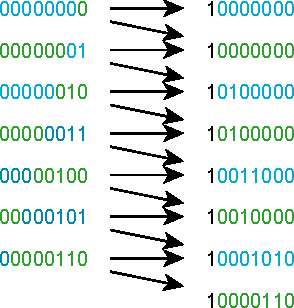
\includegraphics[width=0.3\textwidth]{fig/c3_desenvolvimento/ex3/bit_transf.pdf}
\caption{Transformação nos bytes do arquivo binário para que possam ser transmitidos. À esquerda tem-se os bytes originais e à direita tem-se os bytes transformados.}
\label{fig:ex3:transformacao}
\end{figure}

Após o recebimento de cada pacote da configuração parcial, o programa embarcado o processa fazendo a transformação inversa dos dados e os salva na memória SPI Flash.
Assim como na transformação direta, este processamento é realizado em blocos de 8 bytes, gerando vetores de 7 bytes de dados.

\subsection{Teste}
O teste deste experimento compreende a construção de um sistema microprocessado que carregue os arquivos binários da memória SPI Flash para a memória DDR3, capture as informações relevantes e indique através de GPIO o final do processo.
Este experimento contribuirá para a compreenção do processo de inicialização de memórias não-voláteis e do tratamento do cabeçalho dos arquivos binários.
Usará-se os programas XPS e SDK, que fazem parte do Embedded Development Kit (EDK).

\subsubsection{MicroBlaze}
Utilizou-se o mesmo microcontrolador MicroBlaze construido no experimento passado, não sendo necessária nenhuma modificação.

\subsubsection{SDK}
\todo{Passo a passo do experimento 3 na SDK}

\subsection{Conclusão}
\todo{Explicar como fui para o próximo experimento}
\section{Experimento 4 - Teste da Autoreconfiguração com \textit{Bootloader} Dedicado}
\todo{Descrever o experimento 4}

\subsubsection{Registrador de \textit{Status}}
Este registrador, acessado através de uma sequência predefinida de comandos pela interface ICAPE2 \cite{ug470 - pp108}, informa 

\todo{Explicar como fui para o próximo experimento}
\section{Experimento 5 - Teste da Autoreconfiguração}
\todo{Descrever o experimento 5}
\todo{Explicar como fui para o próximo experimento}

\ifx\compilewholereport\undefined
	\bibliographystyle{plain} 
	%\bibliography{bibliografia.bib}
	\newsavebox\mytempbib\savebox\mytempbib{\parbox{\textwidth}{\bibliography{bibliografia}}}

	\end{document}
\fi